\documentclass[letterpaper]{article}
\usepackage{aaai}
\usepackage{url}
\usepackage{fullpage}
\usepackage{graphicx,curves}
\usepackage{amsmath}
\usepackage{amssymb}
%\usepackage{cmbright}
\usepackage{latexsym}
\usepackage{multirow}
\usepackage[algoruled,vlined,linesnumbered]{algorithm2e}
\usepackage{wrapfig}
\usepackage{pdfsync}
\usepackage{hyperref}

\usepackage[bitstream-charter]{mathdesign}
%\renewcommand*\ttdefault{lmvtt}
\usepackage[T1]{fontenc}
\usepackage{natbib}
\usepackage{booktabs}

\newtheorem{df}{Definition}
\newtheorem{notation}{Notation}
\newtheorem{theorem}{Theorem}
\newtheorem{lemma}{Lemma}[section]
\newtheorem{col}{Corollary}
%\newcommand{\bt}{\begin{theorem}\em}
%\newcommand{\et}{\end{theorem}}
\newcommand{\Qed}{$\blacksquare$}
\newcommand{\qed}{$\Box$}
%\newcommand{\proof}{{\bf Proof. }}
\newcommand{\nin}{\noindent}
\newcommand{\dist}{\operatorname{dist}}
\newcommand{\avg}{\operatorname{avg}}

\newcommand{\citea}[1]{(\citeauthor{#1}, \citeyear{#1})}

\numberwithin{equation}{section}
\numberwithin{theorem}{section}
\numberwithin{lemma}{section}
\numberwithin{df}{section}

\setcounter{secnumdepth}{2} %% this gives us back SECTION NUMBERS!

\DeclareMathOperator*{\argmax}{arg\,max}
\DeclareMathOperator*{\argmin}{arg\,min}

\graphicspath{ {./images/} }

%\usepackage[utf8]{inputenc}
%\usepackage{geometry}
%\usepackage{algorithm}
%\usepackage{algpseudocode}

\global\hyphenpenalty=10000


\title{A Neural Network for Hill-Climbable Sub-goals}

\nocopyright

\author{Zeyi Wang \\
    Department of Computing Science \\ University of Alberta \\
    Edmonton, Alberta, T6G 2E8, Canada \\
    {\texttt{zeyi2@ualberta.ca} }}


\begin{document}

    \maketitle

    \begin{abstract}
        Real-time heuristic search algorithms are most useful for searching tasks that are agent-centered with constrained amount of time and memory resources.
        A common example of this kind of task is pathfinding in modern video games where numbers of entities plan their paths simultaneously.
        Previous work on static map pathfinding focused on using a case base of pre-computed information.
        However, these algorithms always have to face the trade-off between case base spaces, querying time, and performance.
        In this paper, we propose a novel way of building and storing pre-computed information by using a neural network that stores further hill-climbable sub-goals.
        We demonstrate that our method is able to achieve much better performance than LRTA*.

        \href{https://github.com/uduse/neural-network-for-hill-climbling-subgoals}{-> project github link}

    \end{abstract}


    \section{Introduction}\label{sec:introduction}
    Using a case base is common technique in real-time search algorithms for static map pathfinding.
    Algorithms that use a case base include D LRTA* \citea{dlrta}, kNN LRTA* \citea{knnlrta}, and HCDPS \citea{hcdps}.
    All of these algorithms have a offline phase and an online phase.
    On the offline phase, these algorithms pre-compute information and store the pre-computed information into custom data structures.
    On the online phase, these algorithms query their customized data structures by proving the agent's current state and the goal state.
    All of these algorithms have to balance the size of their case bases and their online performance.
    More specifically, as a case base grows larger, the agent is more likely to find a similar case in the case base and thus yield better performance.

    In this paper, we try to replace the use of a case base with the use of a neural network.
    A nice property of neural networks is that a neural network can approximate the mapping of infinitely many inputs and outputs.
    However, the quality of the mapping is heavily dependent on the capacity of the neural network and the amount of training the neural network received.
    We demonstrate that a simple neural network can approximate the mapping between problems and sub-goals to achieve near perfect sub-optimality.

    In our offline phase, we sample random problems from a selected map and compute the corresponding optimal solution paths.
    We extract start, goal, hill-climbable sub-goals from the optimal solution paths as training data.
    We use the training data to train a neural network for a designated number of epochs.

    In our online phase, the agent switches between querying the next sub-goal and trying to hill-climb to the current sub-goal.
    There is no guarantee that the sub-goals provided by the neural network are always hill-climbable.
    To assure that the algorithm is complete, we fall back to an oracle (weighted LRTA*) when the default algorithm fails.

    \section{Problem Formulation}\label{sec:problem-formulation}

    We define a heuristic problem as a directed graph containing a finitely many number of \textit{states} $S$, in which one is the \textit{start} and one is the \textit{goal}
    All \textit{edges} $E$ connecting adjacent states have fixed costs of 1.
    An edge that connects two states always have a reversed edge corresponds to it.
    This also means that the graph is safe to explore.
    The agent has a single \textit{current state} at every time step.
    The agent can take an action by following an edge to change its current state.
    Our \textit{task} is to find a solution given a pair of a start state and a goal state.
    The \textit{solution cost} is the sum of all edge costs of a path the agent can follow to go from the start state to the goal state.
    The algorithm must be complete, which means it must find a solution if there exists one.
    The algorithm can only perform bounded computation to plan a move.
    A \textit{heuristic function} estimate the solution cost between the current state and the goal state.
    We use manhattan distance as the heuristic function.
    The performance of the algorithm is measured in a few ways.
    We measure \textit{offline time} by measuring the time spent on the offline phase in wall clock time.
    We measure the \textit{offline space} by measuring the size of the neural network store on disk.
    We measure \textit{fallback rate} by measuring the percent of time our algorithm uses the fallback algorithm instead.
    We measure the \textit{move time} as the mean time spent on planning between each moves in wall clock time.
    We measure the \textit{neural network time} as the total time spent on retrieving a sub-goal from the neural network in wall clock time,
    including the time spent on converting states to their corresponding indices.
    We measure the \textit{total time} as the sum of move times the task in wall clock time.
    We also measure the \textit{sub-optimality} by taking the ratio between the solution cost of the agent and the optimal solution cost, then minus that number by 1.
    A sub-optimality of 0\% indicates that the solution has the same cost as the optimal solution.
    A sub-optimality of 100\% indicates that the solution cost is twice as much as the optimal solution.


    \section{Related Work}\label{sec:related-work}

    Real-time search algorithms for static map pathfinding usually have two phases.
    In the offline phase, pre-computed information related to the map are store in custom data structures.
    D LRTA* divides a map into regions and use region representatives and region boundaries as sub-goals.
    While HCDPS also divides a map into regions, it does so in a way that states within a region is always mutually hill-climbable to its representative.
    HCDPS is the state-of-the-art on static map pathfinding at the time and have superior performance over D LRTA* in terms of case base size, move time, and sub-optimality.
    Though both D LRTA* and HCDPS set sub-goals, the hill-climbability of HCDPS's sub-goals guarantees its performance.
    D LRTA*, on the other hand, has to run a complete real-time search algorithm to reach the sub-goals.
    As a result, D LRTA* suffers from scrubbing as long as the chosen real-time search algorithm also suffers from scrubbing.
    We draws inspiration from the idea of using hill-climbable sub-goals to reduce scrubbing.
    As a result, we train the neural network so it is most likely to output sub-goals that are hill-climbable.
    kNN LRTA* builds its case base by randomly sampling optimal paths for the map.
    We also build our training data by sampling random optimal paths.
    However, instead of storing the entire pass, we compress the paths using the same method described in HCDPS.
    To guarantee the completeness of our algorithm, we use a weighted LRTA* \citea{wlrta} as our fallback algorithm with a weight of 8.
    We also compare the performance of our algorithm to a weighted LRTA* with a weight of 8.
    We select this algorithm as our fallback and as our baseline because of the time constrain of the project.

    NNRT \citea{nnrt} is the only algorithm we know that uses a neural network in planning.
    However, NNRT uses a neural network to produce next moves, while we produce sub-goals.

    \section{Proposed Approach}\label{sec:proposed-approach}

    \subsection{Offline Phase}

    \subsubsection{Training Data Preparation}

    We first extract all passable tiles from the map as a pool of states $S$.
    We then create an encoding function $\pi$ that maps a given state $s \in S $ to its index in $S$ so that $s = S_{\pi(s)}$.
    We also create a decoding function $\sigma$ that maps a given index back to a state so that $s = \sigma(\pi(s))$.
    We then randomly select a pair of start state $e$ and goal states $g$ with the constraint of $e \neq g$.
    We then compute optimal paths $p^*$ for these pairs using the A* algorithm.
    An optimal path is stored as a sequence of states that includes the start state and the goal state, which means $p^* = e, ~ \dots ~, g$.
    We then use the same algorithm to compute sub-goals as the one used in HCDPS.
    Specifically, given an optimal path $p^*$, we use a binary search to determine the furthest $s_i \in p^*$ that is hill-climbing reachable from $e$.
    We store $s_i$ as a hill-climbable sub-goal $h_1$ and truncate the path $p^*$ up to $s_i$ so we are left with a sub-path of $p^{*'} = s_{i+1}, ~ \dots ~, g$.
    We then recursively apply the same procedure to obtain next sub-goal $h_{2}$ until $h_k = g$.
    We store the indices of the sub-goals so we can represent a path as:
    \[ p^* = e, ~ \dots ~, h_1, ~ \dots ~, h_2, ~ \dots ~, h_k \]
    For each $s_i \in p^*$, we find the next sub-goal $h_i$ by comparing the index values.
    Then the tuple $\left( \pi(s_i), \pi(g), \pi(h_i) \right)$ forms a data point in the training data.
    This way, for a path of length $k$, we can create $k$ data points.

    \subsubsection{Neural Network Training}

    We first define the structure of the neural network.
    Since the inputs are index-based, the first layer of the neural network is an embedding layer that maps an index to a 512 dimensional vector.
    Then the outputs of the embedding layer are connected to a fully connected hidden layer with 512 units.
    The layer has a dropout \citea{dropout} of 0.5 probability and ReLu as the activation function.
    Then this hidden layer is connected to a fully connected output layer with 512 units.
    The output layer uses log Softmax as the activation over the size of pool $|S|$.
    We use Adam \citea{adam} as the optimizer and negative log likelihood as the loss function.

    Our implementation of the training do not separate data preparation and model training.
    Instead, data points are created on the fly, including sampling paths, finding hill-climbable sub-goals, and creating data points.
    This means the time we spend in the offline phase is always proportional to the amount of training the model receives.
    This also means we are not using a fixed set of training data so that the model always use freshly sampled data points for each batch.
    For each batch of samples of size $b$, we use $\pi(s_i), \pi(g)$ as the inputs and $\pi(h_i)$ as the outputs.

    Once the neural network is trained for a desired amount, we save the neural network for future inference.
    Since the output of the neural network is a distribution instead of a single value, we need to use $\argmax$ operator to retrieve the sub-goal that the neural network is most confident of.
    To achieve this, we wrap the neural network $N$ in a function $M$ that returns the sub-goal with the highest score given a start and goal so that:
    \[ M(e, g) = \sigma(\argmax N(\pi(e), \pi(g))) \]

    \subsection{Online Phase}

    The agent follows the procedure \texttt{NNHCS} described in~\ref{alg:nnhcs} to make moves.
    A sub-routine called \texttt{HillClimb} is also defined in~\ref{alg:hill_climb}.
    The fallback algorithm $\Omega$ used is a weighted LRTA* with a weight of 8.

    The agent first queries the neural network for a suitable sub-goal.
    Then, it tries to hill-climb to the sub-goal for at most $c$ steps.
    A cutoff $c$ is used because we find out that queried sub-goals are more accurate when the agent is closer to the goal.
    As a result, applying a cutoff forces the agent to re-think before hill-climbing too far.
    Ideally, the neural network always produces the optimal sub-goals, and the agent always hill-climbs to the goal.
    However, sometimes the neural network makes a mistake, making the agent takes wrong moves.
    If the agent visits a state more than once, we know that the agent must have made a mistake, so we use the fallback algorithm there instead.

    \begin{algorithm*}
        \DontPrintSemicolon
        \label{alg:nnhcs}
        \caption{Neural Network for Hill-Climbing NNHCS($S, E, e, g, M, c$)}

        initialize current state as the start state: $s \leftarrow e$

        initialize visit counts: $\forall s \in S, V_s \leftarrow 0$

        initialize final path as a list: $P \leftarrow [e] $

        initialize the fallback algorithm: $\Omega$

        \While {$s \neq g$}
        {
            \If {$V_s \le 1$}
            {

                query sub-goal: $h \leftarrow M(s, g) $

                \If {$h = s$}
                {
                    increment visit count for current state if not moving: $V_s \leftarrow V_s + 1$
                }

                retrieve hill climb path: $J = \mathit{HillClimb}(S, E, s, h, c)$

                \For {$s' \in J$}
                {
                    increment visit count for climbed states: $V_{s'} \leftarrow V_{s'} + 1$

                    append to final path: $P \leftarrow P \cup [s'] $
                }

            }
            \Else
            {
                take action with the fallback algorithm: $s \leftarrow \Omega(S, E, s, g) $

                increment visit count: $V_{s} \leftarrow V_{s} + 1$

                append to final path: $P \leftarrow P \cup [s'] $
            }

        }

        \Return P

    \end{algorithm*}

    \begin{algorithm*}
        \DontPrintSemicolon
        \label{alg:hill_climb}
        \caption{HillClimb($S, E, e, g, c$)}

        initialize current state as the start state: $s \leftarrow e$

        initialize visited states as a set: $V \leftarrow \{e\}$

        initialize final path as a list: $P \leftarrow [e]$

        \While {$s \neq g \land |P| < c$}
        {
            find the next state: $s' \leftarrow \argmin_{\{s' \in S | \exists E(s, s') \}} \mathit{Manhattan}(s', g) $

            \If {$s' \in V$}
            {
                \Return P
            }
            \Else
            {
                take action: $s \leftarrow s' $

                add state to visited: $V \leftarrow V \cup \{s\} $

                append state to path: $P \leftarrow P \cup [s] $
            }
        }
        \Return P
    \end{algorithm*}


    \section{Theoretical Analysis}\label{sec:theoretical-analysis}

    % Discuss expected properties of your algorithm. For instance, what is the run-time complexity in time and space? Under what assumptions is your algorithm guaranteed to find a solution? If it is a learning algorithm, under which conditions will it converge?

    \subsection{Completeness}\label{subsec:completeness}

    We keep track of the visit counts $V$ and we use a complete fallback algorithm.
    For each state, the agent would try to hill-climb from there at most once.
    As a result, the algorithm completely degrades to the fallback algorithm after at most $|S|$ queries of the neural network.
    Therefore, our algorithm \texttt{NNHCS} is complete.

    \subsection{Offline Time Complexity}\label{subsec:offline-time-complexity}
    We use A* to compute optimal paths, and the complexity of A* is $O(|E|)$.
    We only use four-connected maps so this is equivalent to $O(|S|)$.
    The maximum length of a path in a map is $|S|$.
    For each optimal path, we use binary search to determine the sub-goals, and we at most perform $|S|$ such binary searches.
    For each binary search, we need to verify if the state is hill-climbing reachable from the start state, and this at most takes $|S|$ steps.
    Hence, this step of creating data points runs in $O(|S| * |S| * |S| * \log{|S|}) = O(|S|^3 * \log{|S|})$.
    As a result, the worst case complexity of $|S|$ data points is $O(|S|^3 * \log{|S|})$,
    which means the worst case offline complexity of a single data point is $O(|S|^2 * \log{|S|})$

    \subsection{Offline Space Complexity}\label{subsec:offline-space-complexity}
    Our implementation do not store training data in the memory: we generate them on-the-fly and discard them after being trained on.
    Therefore, the only offline space required is that to store the neural network.
    The size of the neural network is only related to the problem through the number of outputs of the last layer.
    As a result, the offline space complexity is $O(|S|)$.
    For larger problems, the neural network might have to scale more than linearly achieve same relative performance to a baseline algorithm.
    However, how to scale the neural network proportional to the problem size remains unknown.

    \subsection{Online Space Complexity}\label{subsec:online-space-complexity}
    NNHCS needs to load the neural network together with the data of mapping function $\pi$ so the total space complexity is $O(|S| + |S|) = O(|S|)$.
    However, if there are multiple agents searching in the map, only one copy of the neural network is needed.
    Therefore, if there are $K$ agents, the per agent worst-case space complexity is $O(\frac{|S|}{K})$.

    \section{Empirical Evaluation}\label{sec:empirical-evaluation}

    We evaluate NNHCS on the map \texttt{den020d.map}~\ref{fig:map} from \textit{Dragon Age: Origins} (DAO) benchmark \citea{benchmarks}.
    We implemented our algorithm in plain Python and built the neural network using PyTorch \citea{pytorch}.

    \begin{figure*}[h]
        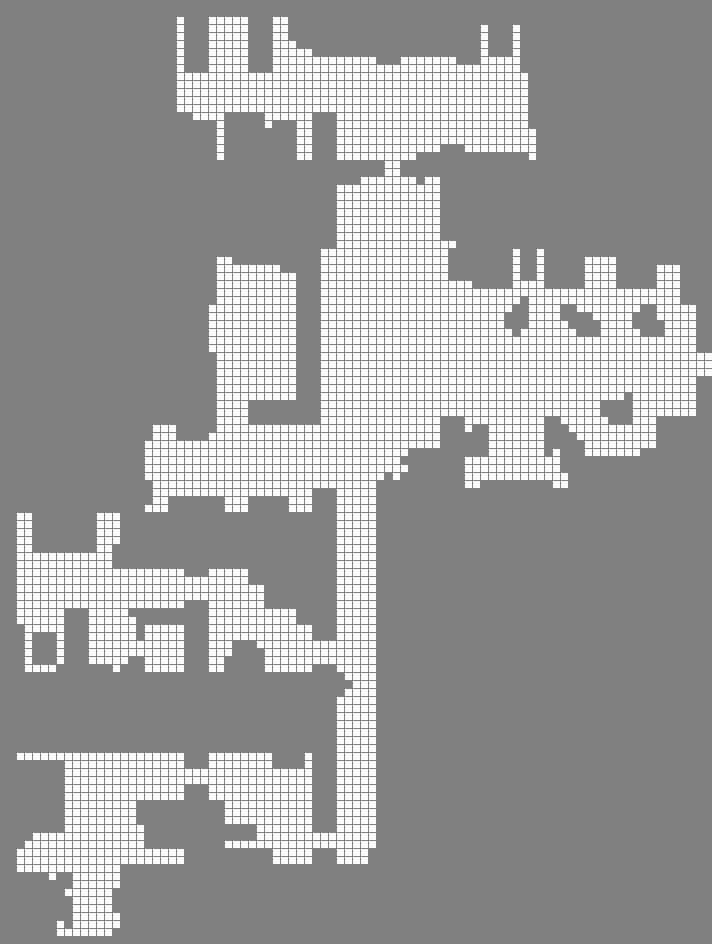
\includegraphics[width=0.5\textwidth]{world.png}
        \caption {\small \texttt{den020d.map} from \textit{Dragon Age: Origins}, grey area are the walls and the white area are the passable tiles.}
        \centering
        \label{fig:map}
    \end{figure*}

    We first evaluated the correctness of the sub-goals provided by the neural network.
    We randomly sampled 256 paths and extract 17784 data points like we described in the previous section~\ref{sec:proposed-approach}.
    We counted the number of errors by comparing the sub-goals provided by the neural network and the actual sub-goals in the data points.
    We found out that only 72\% of the time the neural network finds the correct sub-goal.
    We then evaluated the quality of the mistaken sub-goals.
    For a given data point that the neural network produced a mistaken sub-goal, we first calculate the optimal path cost from the start state to the goal state.
    Second, we add the optimal path cost from the start state to the mistaken sub-goal and the optimal path cost from the sub-goal mistaken sub-goal to the goal state.
    We take the ratio between these two numbers and minus one to get the sub-optimality of the mistaken sub-goal.
    We applied this procedure to all mistaken sub-goals and aggregated the data.
    The average sub-optimality of mistaken sub-goals is 1.70\% with a standard deviation of 36.08\%.
    This means that when the neural network makes a mistake, most likely it will still produce a sub-goal that lies on the optimal path.

    We then compared NNHCS's performance to a weighted LRTA* with a weight of 8.
    We did not compare NNHCS with other algorithm because of the limited time scope of the project.
    We trained the neural network for 100 epochs with roughly 142k data points each epoch.
    We used a single computer with Intel Core i7-9700K Processor and EVGA GTX 970 GPU for training.
    The training process took roughly 15 minutes, including processing other data in the offline phase.

    We only evaluated our result on one trained neural network because the process is too time consuming.
    These results are obtained by generating 2000 random problems from the map and run each algorithm on these problems.
    The results are shown in~\ref{tab:table}.

    \begin{table*}
        \label{tab:table}
        \scriptsize
        \begin{tabular}{|c|c|c|c|c|c|c|c|}
            \hline
            Algorithm & Offline Space (MB) & Offline Time (s) & Fallback (\%) & Move Time (ms) & NN Time (ms) & Total Time (ms) & Sub-optimality (\%) \\
            \hline
            LRTA* (8) & 0 & 0 & 0 & 2.38 $\pm$ 4.872 & 0 & 222.22 $\pm$ 223.83 & 312.21 $\pm$ 520.57 \\
            \hline
            NNHCS & 15 & 938 & 0.42 $\pm$ 2.46 & 3.16 $\pm$ 5.09 & 13.92 $\pm$ 8.03 & 123.12 $\pm$ 20.14 & 1.94 $\pm$ 13.32 \\
            \hline
        \end{tabular}
        \caption{\small Results from 2000 random problems}
    \end{table*}


    As we can see from the table, the fallback is only about 2.5\%, which means 97.5\% of the time the algorithm follows the sub-goals provided by the neural network.
    The move time of NNHCS is higher as expected, since it has to make queries to the neural network.
    However, the total time of NNHCS is lower since it achieves better sub-optimality.
    The time spent on querying the neural network is only a fraction (roughly 11\%) of total time.
    We believe this is due to the fact that the algorithm is written in plain Python, which is slow,
    while the neural network computation is done by a highly optimized third party library.

    NNHCS saves 99 microseconds per problem compared to the weighted LRTA*.
    This means after roughly running 9475 problems, we are break-even on the time we spent on the offline phase and the time we save on the online phase.
    After 9475 problems, the time we spent on the offline phase starts to payoff.
    As more problems are solved by the algorithm, we asymptotically approach the total time ratio of NNHCS and weighted LRTA* and enjoy a near 45\% speed up over weighted LRTA*.

    Check out \href{https://github.com/uduse/neural-network-for-hill-climbling-subgoals/tree/master/temp_images}{link here} to see the algorithm in action.
    The green dot is the start state, the red dot is the goal state, and the purple dot is the sub-goal provided by the neural network.
    When an agent spins around locally, it means the fallback algorithm is taking over.


    \section{Discussion}\label{sec:discussion}

    % Discuss your results with respect to the hypotheses you formulated and the demands of the problem at hand. Do not be shy to admit that you do not understand some of the results you obtained. Leave them as open questions for further research.

    The most surprising fact of NNHCS is that even though it does not have a high accuracy (72\%), it achieves a relatively low sub-optimality (1.9\%).
    This means that even though the neural network does not capture the exact mapping from inputs to sub-goals,
    it does learn about the relationship between inputs and sub-goals.
    In other words, the neural network makes a ``mistake'' because it has seen similar inputs where the start state and the goal state are similar.
    However, the sub-goal that similar inputs use is likely to be a good sub-goal to the current problem as well.
    Notice that the neural network does not explicitly receive information about adjacency of states.
    The inputs and outputs are both represented as indices, and the inputs is directly translated to a 512 dimensional vector in embedding layer.
    This means that the neural network learned about adjacency of states somehow, and that information of adjacency is most likely to be stored in the embedding layer.
    We tried to use a three dimensional embedding layer to train a neural network, then plot the embedding layer to the map as RGB values.
    We observed some localities (similar colors grouped together) but these patterns are not obvious and are hard to draw a conclusion from.
    One potential reason is that the neural network is not sufficiently trained on a small embedding layer of 3 dimensions.
    If we compress the embedding layer of our final neural network into 3 dimensions (e.g., using a variance auto encoder), the results may be more informative.


    \section{Conclusion and Future Work Directions}\label{sec:future-work}

    In this work we have presented NNHCS, the first algorithm on static map pathfinding that uses a neural network.
    We demonstrated the algorithm is capable of achieve near perfect sub-optimality on a small map.
    The potential of the algorithm is by no means fully explored due to the time constraint.
    However, we envision two promising directions to further explore the algorithm:

    (1) The concept of using information in an embedding layer also appeared in the FastMap algorithm \citea{fastmap}.
    The difference is that the FastMap algorithm uses a manually computed embedding layer while NNHCS uses an embedding layer that is learned by a neural network.
    These two approaches share the same idea of ``relating states to other states in a multi-dimensional space''.
    The FastMap algorithm is the state-of-the-art on static map pathfinding, and NNHCS also shows a near optimal performance in sub-optimality.
    This means that both algorithms can complete their task relatively well using the embedding layer.
    Then the question we would like to ask is that, can they share their embedding layer with each other and achieve even better performance?
    Or, can we create an embedding layer that encode enough information so both these two algorithms can use the same embedding layer with some modifications to the algorithms?
    This idea of accomplishing different tasks with the same embedding layer is proven successful in the natural language processing field (e.g., BERT \citea{bert}).
    If we pre-train a good enough embedding layer for states in a given map or a pool of maps, maybe we can accomplish various tasks related to the map.
    The FastMap algorithm may use the embedding layer for heuristic values, and the NNHCS algorithm may use the embedding layer to find optimal sub-goals.
    Pre-training an embedding layer for various tasks is an avenue of future research.

    (2) One of our biggest concern of the algorithm was that our approach is not cost-sensitive.
    This means the loss of a good sub-goal is the same as a wrong sub-goal as long as they are not the optimal sub-goal.
    We thought this will lead to poor generalizing of the neural network.
    However, our experiment showed that even though neural network makes mistakes, most of their mistakes are still optimal.
    Our guess is that the neural network learned about cost-sensitive indirectly through locality.
    We believe that if we make the loss function cost-sensitive,
    we can further increase the performance of our algorithm by either reducing sub-optimality or reducing training time to achieve the same sub-optimality.

    \newpage

    \section*{Acknowledgments}

    % Acknowledge any help you already received.
    I gratefully acknowledge the help by Vadim Bulitko, without which the present study could not have been completed.
    I also gratefully acknowledge the support by Levi Lelis who extended his project deadline so I can make this project more complete.

    \bibliography{projectReport}
    \bibliographystyle{aaai}

\end{document}
